%!TEX program = xelatex
\documentclass[titlepage,oneside]{ctexart}
\usepackage{ecustpc}
\title{ECUST Programming Contest 2026 Fall -- Problem Statements}
\author{ECUSTPC 2026 Fall Jury}
\date{September 29, 2026}

\begin{document}
\setcontestheader{ECUST Programming Contest 2026 Fall}{September 29, 2026}
\pagestyle{fancy}
\setlength{\headheight}{25.3186pt}
\begin{titlepage}
\begin{center}
    \huge{\textbf{ECUST Programming Contest 2026 Fall}} \\[10pt]
    \huge{Official Contest -- Problem Statements} \\[10pt]
    \Large{September 29, 2026, 13:00--18:00}
\end{center}
\vspace{2em}
{\large\BF{Problem List}}
\begin{table}[htbp]
\begin{center}
\small
\begin{tabular}{ccccc}
\toprule
Problem & Title & Limits & Note \\
\midrule
\myboxi{\BF{\TT{A}}} & \BF{Synecdoche, New York} & 2s/1GB & \\
\myboxii{\BF{\TT{B}}} & \BF{AIMC Lab} & 2s/1GB & \\
\myboxiii{\BF{\TT{C}}} & \BF{Split in Two 2} & 2s/1GB & \\
\myboxiv{\BF{\TT{D}}} & \BF{Unit Distance!?} & 2s/1GB & \\
\myboxv{\BF{\TT{E}}} & \BF{Eradication} & 4s/1GB & \\
\myboxvi{\BF{\TT{F}}} & \BF{Convex Hull} & 2s/1GB & \\
\myboxvii{\BF{\TT{G}}} & \BF{Beyond the Stars} & 8s/1GB & Communication \\
\myboxviii{\BF{\TT{H}}} & \BF{Ordinary Offensive Magic} & 2s/1GB & \\
\myboxix{\BF{\TT{I}}} & \BF{Shooting Stars} & 1s/1GB & \\
\myboxx{\BF{\TT{J}}} & \BF{Time Trouble 2} & 1s/1GB & \\
\myboxxi{\BF{\TT{K}}} & \BF{Aeonglass} & 2s/1GB & \\
\myboxxii{\BF{\TT{L}}} & \BF{In Filtration 3} & 2s/1GB & \\
\myboxxiii{\BF{\TT{M}}} & \BF{Witch Trial} & 6s/1GB & \\
\bottomrule
\end{tabular}
\end{center}
\end{table}

This booklet contains 13 problems. If pages are missing, contact a volunteer immediately.

Please read the contest rules and technical rules included with the contest files.

Do not open the booklet or touch the mouse or keyboard before the contest begins.

Black-and-white printing may obscure information conveyed by color.

\textit{The italic text before each problem statement is flavor text and is unrelated to the problem. It is intentionally left untranslated.}
\end{titlepage}

\linespread{1.0}
\setlength{\parskip}{0\baselineskip}
\normalsize
\newpage
\setcounter{page}{1}

\section[A. Synecdoche, New York]{\myboxi{      \BF{\TT{A}}} Synecdoche, New York}

\textit{Time limit}   2 seconds

\textit{Memory limit} 1 Gigabyte

\textit{Input} \qquad standard input

\textit{Output} \qquad standard output


\begin{quote}
	\textit{And they say there is no fate, but there is, it's what you create.}

	\textit{And even though the world goes on for eons and eons...}

	\textit{...you are only here for a fraction of a fraction of a second.}
\end{quote}

\subsection{Problem Statement}

Caden has come to understand ``fate'' in his own way. Leaving theater behind, he wants to use a string to represent his life through synecdoche. But in seeking a pure, original expression true to himself, he again falls into an infinite loop of self-reference. This time, Caden leaves the choice to you: portray his life for him.

Caden's synecdoche is a string $T$ of length $L$. We call $T$ \BF{valid} if and only if all three conditions below hold:

\begin{enumerate}
	\item $T$ consists only of lowercase English letters.
	\item For every $i = 1, 2, \ldots, K$, the character of $T$ at position $p_i$ must equal the given character $c_i$, where $1 \le p_i \le L$ and $c_i$ is a lowercase letter.
	\item For every $i = 1, 2, \ldots, N$, the given string $s_i$ must \BF{not} occur as a contiguous substring of $T$.
\end{enumerate}

Given $L$, $K$ position constraints $(p_i,c_i)$, and $N$ forbidden substrings $s_i$, count all valid strings $T$. Output the answer modulo $998\,244\,353$.

\subsection{Input}

The first line contains three integers $L$, $K$, and $N$ ($1 \le L \le 10^{18}$, $0 \le K \le 500$, $0 \le N \le 50$): the string length, the number of position constraints, and the number of forbidden substrings.

Each of the next $K$ lines contains an integer $p_i$ and a lowercase letter $c_i$ ($1 \le p_i \le L$), describing a position constraint. All $p_i$ are distinct.

Each of the next $N$ lines contains a nonempty string $s_i$, describing a forbidden substring.

The sum of the lengths of all $s_i$ does not exceed $100$; that is, $\sum_{i=1}^N \vert{}s_i\vert{} \le 100$.

\subsection{Output}

Output one integer for each test case: the number of valid strings modulo $998\,244\,353$.

\subsection{Sample 1}

\begin{minipage}{\linewidth}
	\begin{minipage}[t]{0.49\linewidth}
		\begin{lstlisting}[title=\texttt{standard input}]
3 1 1
2 b
ab
\end{lstlisting}
	\end{minipage}
	\begin{minipage}[t]{0.49\linewidth}
		\begin{lstlisting}[title=\texttt{standard output}]
650
\end{lstlisting}
	\end{minipage}
\end{minipage}

\subsection{Sample 2}

\begin{minipage}{\linewidth}
	\begin{minipage}[t]{0.49\linewidth}
		\begin{lstlisting}[title=\texttt{standard input}]
10 2 2
3 a
5 c
abc
dcabe
\end{lstlisting}
	\end{minipage}
	\begin{minipage}[t]{0.49\linewidth}
		\begin{lstlisting}[title=\texttt{standard output}]
113392371
\end{lstlisting}
	\end{minipage}
\end{minipage}


\subsection{Sample 1 Explanation}

The string has length $3$, its second character must be \TT{b}, and it must not contain \TT{ab}. Valid strings have the form \TT{?b?}; the first character can be any lowercase letter except \TT{a}. There are $25 \times 26 = 650$ such strings.


\newpage
\section[B. AIMC Lab]{\myboxii{      \textbf{\texttt{B}}} AIMC Lab}

\textit{Time limit}   2 seconds

\textit{Memory limit} 1 Gigabyte

\textit{Input} \qquad standard input

\textit{Output} \qquad standard output


\begin{quote}
	\textit{街灯璀璨，可我日渐透明。}
\end{quote}

\subsection{Problem Statement}

Your AIMC Lab has developed an entirely new three-dimensional quantum matrix!

Consider a three-dimensional grid of size $N \times M \times H$, with coordinates $1 \le x \le N$, $1 \le y \le M$, and $1 \le z \le H$. A qubit occupies every integer grid point. Let $(x_u,y_u,z_u)$ be the coordinates of qubit $u$.

For any two qubits $u$ and $v$, define their \textbf{squared spatial distance} as
$$
d^2(u, v) = (x_u - x_v)^2 + (y_u - y_v)^2 + (z_u - z_v)^2.
$$

The system has eight energy matrices $A_{D,c}$, each of size $N \times M \times H$, indexed by integers $0 \le D \le 3$ and $0 \le c \le 1$.

You may initialize each qubit to either basis state $|0\rangle$ or $|1\rangle$. Its corresponding basis-state value is $c_P=0$ or $c_P=1$.

After initialization, the total energy is calculated as follows:

\begin{itemize}
	\item For each integer pair $0 \le D \le 3$, $0 \le c \le 1$, qubit $P$ gains $A_{D,c}(x_P,y_P,z_P)$ energy if and only if:
	\begin{itemize}
		\item The basis-state value of $P$ satisfies $c_P=c$.
		\item For every qubit $Q$ with $d^2(P,Q)=D$, the value $c_P+c_Q+D$ is even.
	\end{itemize}
\end{itemize}

As the chief scientist of AIMC Lab, initialize every qubit to a basis state so that the system's total energy is maximized. Output this maximum energy.

\subsection{Input}

The first line contains three integers $N$, $M$, and $H$ ($1 \le N,M,H \le 20$), the grid dimensions.

The data for the eight energy matrices $A_{D,c}$ follow in lexicographic order of $(D,c)$.

Each matrix consists of $N$ blocks. Each block has $M$ lines, each containing $H$ integers. Blocks are separated by blank lines.

The $z$-th number in the $y$-th line of the $x$-th block is the energy at $(x,y,z)$. All energy values satisfy $A_{D,c}(x_P,y_P,z_P) \in [0,10^9]$.

\subsection{Output}

Output one integer: the maximum total energy the system can achieve.

\subsection{Sample 1}

\begin{minipage}{\linewidth}
	\begin{minipage}[t]{0.49\linewidth}
		\begin{lstlisting}[title=\texttt{standard input}]
1 1 1
3

5

100

200

1000

2000

50

60
\end{lstlisting}
	\end{minipage}
	\begin{minipage}[t]{0.49\linewidth}
		\begin{lstlisting}[title=\texttt{standard output}]
2265
\end{lstlisting}
	\end{minipage}
\end{minipage}


\subsection{Sample 1 Explanation}

The grid contains only one qubit, at $(1,1,1)$.

Initializing it to $|1\rangle$ gives $A_{0,1}(1,1,1)+A_{1,1}(1,1,1)+A_{2,1}(1,1,1)+A_{3,1}(1,1,1)=5+200+2000+60=2265$, which is optimal.

\subsection{Sample 2}

\begin{minipage}{\linewidth}
	\begin{minipage}[t]{0.49\linewidth}
		\begin{lstlisting}[title=\texttt{standard input}]
2 2 2
1 1
1 1

1 1
1 1

0 0
0 0

0 0
0 0

0 0
0 0

0 0
0 0

0 0
0 0

0 0
0 0

10 10
10 10

10 10
10 10

0 0
0 0

0 0
0 0

0 0
0 0

0 0
0 0

0 0
0 0

0 0
0 0
\end{lstlisting}
	\end{minipage}
	\begin{minipage}[t]{0.49\linewidth}
		\begin{lstlisting}[title=\texttt{standard output}]
88
\end{lstlisting}
	\end{minipage}
\end{minipage}


\subsection{Sample 2 Explanation}

Initialize all $8$ qubits of the $2 \times 2 \times 2$ grid to $|0\rangle$.

\begin{itemize}
	\item Each qubit gains $1$ energy from $A_{0,0}$, for a total of $8$.
	\item All qubits at squared distance $2$ are also in state $|0\rangle$, so each qubit gains $10$ from $A_{2,0}$, for a total of $80$.
\end{itemize}

The total energy is $8+80=88$. This can be shown to be the maximum.

\newpage
\section[C. Split in Two 2]{\myboxiii{      \BF{\TT{C}}} Split in Two 2}

\textit{Time limit}   2 seconds

\textit{Memory limit} 1 Gigabyte

\textit{Input} \qquad standard input

\textit{Output} \qquad standard output


\begin{quote}
	\textit{别在昨日里频频回首，说什么将寂寞对半分担。}
\end{quote}

\subsection{Problem Statement}

You are given two arrays $a$ and $b$, each of length $n$.

Choose any $k \in [0,n]$ and concatenate the first $k$ elements of $a$ with the last $n-k$ elements of $b$ to form a new array of length $n$.

Select exactly $m$ pairwise nonadjacent elements from the new array. Let $p$ be the smallest selected element. Maximize $p$.

\subsection{Input}

The first line contains an integer $T$ ($1 \le T \le 10^4$), the number of test cases.

The first line of each test case contains two integers $n$ and $m$ ($1 \le m \le \lceil \frac n2 \rceil \le n \le 2 \times 10^5$): the array length and the number of elements to select.

The second line contains $n$ integers $a_1,a_2,\ldots,a_n$ ($-10^9 \le a_i \le 10^9$).

The third line contains $n$ integers $b_1,b_2,\ldots,b_n$ ($-10^9 \le b_i \le 10^9$).

The sum of $n$ over all test cases does not exceed $2 \times 10^5$.

\subsection{Output}

For each test case, output one integer: the maximum possible value of $p$.

\subsection{Sample 1}

\begin{minipage}{\linewidth}
	\begin{minipage}[t]{0.49\linewidth}
		\begin{lstlisting}[title=\texttt{standard input}]	
2
5 2
5 4 3 2 1
1 2 3 4 5
9 5
1 1 4 5 1 4 1 9 1
9 9 8 2 4 4 3 5 3
\end{lstlisting}
	\end{minipage}
	\begin{minipage}[t]{0.49\linewidth}
		\begin{lstlisting}[title=\texttt{standard output}]
5
3
\end{lstlisting}
	\end{minipage}
\end{minipage}

\subsection{Sample 1 Explanation}

In the first test case, choosing $k=4$ gives $[5,4,3,2,5]$. Select the first and fifth elements; their minimum is $5$, which is optimal.

\newpage
\section[D. Unit Distance!?]{\myboxiv{      \BF{\TT{D}}} Unit Distance!?}

\textit{Time limit}   2 seconds

\textit{Memory limit} 1 Gigabyte

\textit{Input} \qquad standard input

\textit{Output} \qquad standard output


\begin{quote}
	\textit{最后跳支舞吧。}

	\textit{在魔都的远郊，}

	\textit{在化工强校的信息楼，}

	\textit{在这个光怪陆离的}

	\textit{革命前夜。}
\end{quote}

\subsection{Problem Statement}

Construct a set of $n$ points in the Euclidean plane such that:

\begin{itemize}
	\item The absolute values of both coordinates of every point are at most $10^5$;
	\item Each coordinate of every point becomes an integer when multiplied by $10^{13}$;
	\item The distance between any two points is at least $10^{-4}$;
	\item At least $\left\lfloor \frac12 n\log_2 n-n \right\rfloor$ distinct unordered pairs of points have distance in $[1-10^{-9},1+10^{-9}]$.
\end{itemize}


\subsection{Input}

The first line contains an integer $T$ ($1 \le T \le 100$), the number of test cases.

Each test case contains one integer $n$ ($2 \le n \le 5000$), the number of points to construct.

The sum of $n$ over all test cases does not exceed $5000$.

\subsection{Output}

For each test case, output $n$ lines. The $i$-th line contains two integers $X_i,Y_i$ ($-10^{18} \le X_i,Y_i \le 10^{18}$), representing the actual point $\left(\frac{X_i}{10^{13}},\frac{Y_i}{10^{13}}\right)$.

Your output is accepted if and only if it satisfies this format and all four conditions above.

If several valid constructions exist, output any one of them.

\subsection{Sample 1}

\begin{minipage}{\linewidth}
	\begin{minipage}[t]{0.49\linewidth}
		\begin{lstlisting}[title=\texttt{standard input}]
1
3
\end{lstlisting}
	\end{minipage}
	\begin{minipage}[t]{0.49\linewidth}
		\begin{lstlisting}[title=\texttt{standard output}]
0 0
10000000000000 0
5000000000000 8660254038000
\end{lstlisting}
	\end{minipage}
\end{minipage}


\subsection{Sample 1 Explanation}

In the first test case, the actual coordinates are:

\[
	(x_1, y_1) = (0, 0), (x_2, y_2) = (1, 0), (x_3, y_3) = (0.5, 0.8660254038)
\]

The first three conditions are easy to verify. The pairwise distances are:

\[d_{12} = 1, d_{13} = d_{23} = 1.000000000013476527219909191607\ldots \approx 1 + 1.3476 \times 10^{-11} \]

Thus every pairwise distance is within the allowed tolerance of $1$, satisfying the fourth condition.

% \subsection{提示}

% 当 $n = 5000$ 时 $\left\lfloor \frac{1}{2}n\log_2 n - n \right\rfloor = 25719$。

\newpage
\section[E. Eradication]{\myboxv{      \BF{\TT{E}}} Eradication}

\textit{Time limit}   4 seconds

\textit{Memory limit} 1 Gigabyte

\textit{Input} \qquad standard input

\textit{Output} \qquad standard output


\begin{quote}
	\textit{我们终于等来了黎明，可这座城的}根除\textit{了记得黑夜，似乎什么也没能留下。}
\end{quote}

\subsection{Problem Statement}

We often simplify the square root of a large integer into radical form; for example, $\sqrt{432}=12\sqrt3$.

Define the number-theoretic function $f(n)=\min\{a \mid n=ab^2,\ a,b\in\mathbb N\}$ on $\N$. In other words, $f(n)$ is the smallest natural number $a$ satisfying the equation. Such an $a$ always exists.

You are given $q$ queries, each specifying $l$ and $r$. For each query, find $\sum_{i=l}^r f(i)$ modulo $998\,244\,353$.

\subsection{Input}

The first line contains an integer $q$ ($1 \le q \le 500$), the number of queries.

Each of the next $q$ lines contains two integers $l$ and $r$ ($1 \le l \le r \le 10^{12}$), specifying a query interval.

\subsection{Output}

For each query, output one integer: $\sum_{i=l}^r f(i)$ modulo $998\,244\,353$.

\subsection{Sample 1}

\begin{minipage}{\linewidth}
	\begin{minipage}[t]{0.49\linewidth}
		\begin{lstlisting}[title=\texttt{standard input}]
4
432 432
1 10
10 15
1 100000000
\end{lstlisting}
	\end{minipage}
	\begin{minipage}[t]{0.49\linewidth}
		\begin{lstlisting}[title=\texttt{standard output}]
3
38
66
651260790
\end{lstlisting}
	\end{minipage}
\end{minipage}


\subsection{Sample 1 Explanation}

For the second and third queries, the corresponding values of $f$ are:

\[
\begin{array}{c|ccccccccccccccc}
n
&1&2&3&4&5&6&7&8&9&10&11&12&13&14&15\\
\hline
f(n)
&1&2&3&1&5&6&7&2&1&10&11&3&13&14&15
\end{array}
\]

In particular, the third query gives
\[
	\sum_{i = 10}^{15}f(i) = f(10) + f(11) + f(12) + f(13) + f(14) + f(15) = 10 + 11 + 3 + 13 + 14 + 15 = 66.
\]



\newpage
\section[F. Convex Hull]{\myboxvi{      \BF{\TT{F}}} Convex Hull}

\textit{Time limit}   2 seconds

\textit{Memory limit} 1 Gigabyte

\textit{Input} \qquad standard input

\textit{Output} \qquad standard output


\begin{quote}
	\textit{我知道既不是凸包也不是凹包的我为什么要哭的。因为我其实是一只豆包。}
\end{quote}

\subsection{Problem Statement}

You are given $n$ quadratic inequalities, each of the form

$$
a_i x^2 + b_i x + c_i  >  0
$$

Determine whether there is an \BF{integer} $x$ satisfying all $n$ inequalities simultaneously.

\subsection{Input}

The first line contains an integer $T$ ($1 \le T \le 10^4$), the number of test cases.

The first line of each test case contains an integer $n$ ($1 \le n \le 2 \times 10^5$), the number of inequalities.

Each of the next $n$ lines contains three integers $a_i,b_i,c_i$ ($-10^5 \le a_i \le -1$, $-10^5 \le b_i,c_i \le 10^5$), the coefficients of the $i$-th inequality.

The sum of $n$ over all test cases does not exceed $2 \times 10^5$.

\subsection{Output}

For each test case, output \TT{YES} if such an integer $x$ exists, or \TT{NO} otherwise.

The answer is case-insensitive; for example, \TT{yes}, \TT{YES}, \TT{Yes}, and \TT{YeS} are all accepted as affirmative answers.

\subsection{Sample 1}

\begin{minipage}{\linewidth}
	\begin{minipage}[t]{0.49\linewidth}
		\begin{lstlisting}[title=\texttt{standard input}]
5
2
-1 0 4
-1 4 -3
3
-1 100000 0
-1 202 10000
-2 400 19998
2
-1 2 0
-1 0 -1
2
-100000 0 100000
-1 0 4
2
-1 2 0
-1 4 -3

\end{lstlisting}
	\end{minipage}
	\begin{minipage}[t]{0.49\linewidth}
		\begin{lstlisting}[title=\texttt{standard output}]
NO
YES
NO
YES
NO
\end{lstlisting}
	\end{minipage}
\end{minipage}


\subsection{Sample 1 Explanation}

In the second test case, $x=100$ satisfies all three inequalities, so an integer solution exists.

\newpage
\section[G. Beyond the Stars]{\myboxvii{      \textbf{\texttt{G}}} Beyond the Stars}

\textit{Time limit}   8 seconds

\textit{Memory limit} 1 Gigabyte

\textit{Input} \qquad standard input

\textit{Output} \qquad standard output


\begin{quote}
	\textit{今夜天空深远宁静，我们望的是同一颗星星吗？}
\end{quote}

\textbf{This is a communication problem. Pay attention to its unusual constraints.}

\subsection{Problem Statement}

That was long ago, in a past forgotten by all of ECUST\ldots

In that forgotten age, Zhulin and Qianwai fought side by side, lived together, and gazed up at the same stars. Later, sand buried their language, oceans severed their roads, and even their names faded from history. Only the vast, silent star chart above them remained: public, radiant, and unchanging. Yet nobody knew which stars they had once quietly joined into a message.

This problem has $20$ test cases.

You are given an undirected graph $G=(V,E)$ with $|V|=2000$ and $|E|=43\,600$. It has no multiple edges or self-loops and is generated as follows. Initially, $G$ has $|V|$ vertices and no edges. Then, $|E|$ times, the generator uniformly chooses one of the vertex pairs not yet joined by an edge and adds an undirected edge between them.

Your program will be run twice:

\textbf{First run}

In the first run, you play Zhulin. Choose and output $n$ induced four-cycles in $G$. They may share vertices.

\begin{itemize}
	\item \textbf{Definition of an induced four-cycle:} Choose $4$ vertices of $G$ that have \textbf{exactly} $4$ edges among them, forming a simple cycle. In particular, there are no diagonals.
\end{itemize}

\textbf{Second run}

In the second run, you play Qianwai. The judge has your complete output from the first run. For each of $q$ queries, it selects one of your four-cycles, deletes one of its vertices, and gives you the other three vertex numbers. Report the index of the four-cycle in Zhulin's output from which they came.

\subsection{Input}

\textbf{First run}

The first line contains the string \texttt{send}.

The second line contains an integer $n$ ($n=200\,000$), the number of induced four-cycles you must output.

The third line contains two integers $|V|$ and $|E|$.

Each of the next $|E|$ lines contains two integers $u,v$, indicating an undirected edge between vertices $u$ and $v$ ($1 \le u,v \le |V|$).

\textbf{Second run}

The first line contains the string \texttt{receive}.

The second line contains two integers $|V|$ and $|E|$.

Each of the next $|E|$ lines contains two integers $u,v$, indicating an undirected edge between vertices $u$ and $v$ ($1 \le u,v \le |V|$).

Line $|E|+3$ contains an integer $q$ ($q=4n$), the number of received vertex sets.

Each of the next $q$ lines contains $3$ integers: the vertices remaining after the judge removes one vertex from a four-cycle in your first-run output.

\subsection{Output}

\textbf{First run}

Output $n$ lines. Line $i$ contains four integers $v_1,v_2,v_3,v_4$, the vertices of the $i$-th induced four-cycle.

\textbf{Second run}

Output $q$ lines. For each received vertex set, output an integer $i$ ($1 \le i \le n$), the index of its four-cycle.

\subsection{Sample 1}

\textbf{First run}

\begin{minipage}{\linewidth}
	\begin{minipage}[t]{0.49\linewidth}
		\begin{lstlisting}[title=\texttt{standard input}]
send
200000
2000 43600
29 1973
228 1127
...
92 573
\end{lstlisting}
	\end{minipage}
	\begin{minipage}[t]{0.49\linewidth}
		\begin{lstlisting}[title=\texttt{standard output}]
1 174 613 1323
1 955 1683 1755
...
1390 1615 1683 1777
\end{lstlisting}
	\end{minipage}
\end{minipage}

\textbf{Second run}

\begin{minipage}{\linewidth}
	\begin{minipage}[t]{0.49\linewidth}
		\begin{lstlisting}[title=\texttt{standard input}]
receive
2000 43600
29 1973
228 1127
...
92 573
800000
46 1297 1949
1056 1275 1454
...
387 1289 1533
\end{lstlisting}
	\end{minipage}
	\begin{minipage}[t]{0.49\linewidth}
		\begin{lstlisting}[title=\texttt{standard output}]
17713
191947
...
118231
\end{lstlisting}
	\end{minipage}
\end{minipage}


\subsection{Sample 1 Explanation}

Parts of the sample are omitted because the complete data is too large.



\newpage
\section[H. Ordinary Offensive Magic]{\myboxviii{      \textbf{\texttt{H}}} Ordinary Offensive Magic}

\textit{Time limit}   2 seconds

\textit{Memory limit} 1 Gigabyte

\textit{Input} \qquad standard input

\textit{Output} \qquad standard output


\begin{quote}
	\textit{``Zoltraak.''}
\end{quote}

\subsection{Problem Statement}

Consider an $n \times m$ grid. Each cell has one of three states:

\begin{enumerate}
	\item \texttt{/} (forward-slash mirror): reflects on both sides. A ray turns $90^\circ$, connecting the top with the left and the bottom with the right.
	\item \texttt{\textbackslash} (backslash mirror): reflects on both sides. A ray turns $90^\circ$, connecting the top with the right and the bottom with the left.
	\item \texttt{.} (empty cell): contains no obstacle. A ray passes straight through, connecting the top with the bottom and the left with the right.
\end{enumerate}

Initially, some cells contain fixed \texttt{/} or \texttt{\textbackslash} mirrors; the rest are empty. You may \textbf{leave each initially empty cell empty}, \textbf{replace it with a \texttt{/} mirror}, or \textbf{replace it with a \texttt{\textbackslash} mirror}.

The outside boundary of the grid consists of $2(n+m)$ unit-length segments. A ray may enter or leave only perpendicularly through the midpoint of one of these segments.

Given an entry point and a target exit point, determine whether the grid can be filled legally so that a ray entering at the specified point, after straight-line travel and reflections, exits at exactly the target point.

If possible, output a valid completed grid that \textbf{minimizes the number of cells traversed} by the ray from the entry point to the target exit point. Count one traversal each time the ray enters a cell; repeated visits to the same cell are counted separately. If there are multiple optimal completions, output any of them. Otherwise, report that it is impossible.

\subsection{Input}

The first line contains an integer $T$ ($1 \le T \le 100$), the number of test cases.

The first line of each test case contains two integers $n,m$ ($1 \le n \times m \le 2 \times 10^5$), the numbers of rows and columns.

Each of the next $n$ lines contains a string of length $m$ describing the initial grid. Here \texttt{/} is a forward-slash mirror, \texttt{\textbackslash} is a backslash mirror, and \texttt{.} is an empty cell.

The next line contains four space-separated values $d_1,p_1,d_2,p_2$. The first pair specifies the entry point, and the second specifies the target exit point:

\begin{itemize}
	\item Each of $d_1,d_2$ is one of U, D, L, R, denoting the top, bottom, left, or right boundary, respectively.
	\item Each of $p_1,p_2$ is a positive integer specifying the midpoint of the outer edge of the $p$-th boundary cell. On U or D, $p$ is a column number ($1 \le p \le m$); on L or R, it is a row number ($1 \le p \le n$).
\end{itemize}

It is guaranteed that $(d_1,p_1) \ne (d_2,p_2)$.

The sum of $n \times m$ over all test cases does not exceed $2 \times 10^5$.

\subsection{Output}

For each test case, if a valid completion exists, output $n$ lines of length $m$ describing a completion that minimizes the number of cells traversed. If there are multiple optimal completions, output any of them. Do not output the minimum number of traversals. Otherwise, output \texttt{IMPOSSIBLE}.

A backslash must usually be escaped: \texttt{\textbackslash\textbackslash} outputs \texttt{\textbackslash}.

\subsection{Sample 1}

\begin{minipage}{\linewidth}
	\begin{minipage}[t]{0.49\linewidth}
		\begin{lstlisting}[title=\texttt{standard input}]
3
2 2
..
..
L 1 U 2
4 4
/\/\
/\/.
....
./..
L 2 L 4
4 4
/\/\
/\/.
..\/
./..
L 2 L 4
\end{lstlisting}
	\end{minipage}
	\begin{minipage}[t]{0.49\linewidth}
		\begin{lstlisting}[title=\texttt{standard output}]
./
..
/\/\
/\//
.//.
./..
IMPOSSIBLE
\end{lstlisting}
	\end{minipage}
\end{minipage}


\subsection{Sample 1 Explanation}

In the first test case, the ray enters from the left edge of row $1$ and travels right. It passes through the empty cell $(1,1)$, turns upward at the \texttt{/} mirror in $(1,2)$, and exits through the top edge of column $2$.

This completion traverses $2$ cells, which is the minimum possible.

\newpage
\section[I. Shooting Stars]{\myboxix{      \BF{\TT{I}}} Shooting Stars}

\textit{Time limit}   1 second

\textit{Memory limit} 1 Gigabyte

\textit{Input} \qquad standard input

\textit{Output} \qquad standard output


\begin{quote}
	\textit{在燥热的季节，一颗流星划过天际，留下光亮的拖尾。}
	
	\textit{我循着光奔跑的那个夜晚，便是故事的开端。}
\end{quote}

\subsection{Problem Statement}

There are $n$ crystals numbered $1$ through $n$ from left to right. Crystal $i$ initially contains $a_i$ units of energy. You may collect all $n$ crystals in any order.

When you collect crystal $i$:

\begin{itemize}
	\item You add its current energy to your total score.
	\item If crystals $i-1$ and $i+1$ exist and have not yet been collected, their energies each change sign.
\end{itemize}

The crystals' numbers do not change as you collect them.

What is the maximum total score after collecting all $n$ crystals?

\subsection{Input}

The first line contains an integer $T$ ($1 \le T \le 10^4$), the number of test cases.

The first line of each test case contains an integer $n$ ($1 \le n \le 2 \times 10^5$), the number of crystals.

The second line contains $n$ integers $a_1,a_2,\ldots,a_n$ ($-10^9 \le a_i \le 10^9$), their initial energies.

The sum of $n$ over all test cases does not exceed $2 \times 10^5$.

\subsection{Output}

For each test case, output one integer: the maximum possible total score.

\subsection{Sample 1}

\begin{minipage}{\linewidth}
	\begin{minipage}[t]{0.49\linewidth}
		\begin{lstlisting}[title=\texttt{standard input}]
2
5
1 2 3 4 5
9
9 -9 8 -2 4 -4 3 -5 3
\end{lstlisting}
	\end{minipage}
	\begin{minipage}[t]{0.49\linewidth}
		\begin{lstlisting}[title=\texttt{standard output}]
15
47
\end{lstlisting}
	\end{minipage}
\end{minipage}

\subsection{Sample 1 Explanation}

In the first test case, collecting crystals in the order $3 \to 5 \to 1 \to 2 \to 4$ gives a score of $15$. This is optimal.

\newpage
\section[J. Time Trouble 2]{\myboxx{      \textbf{\texttt{J}}} Time Trouble 2}

\textit{Time limit}   1 second

\textit{Memory limit} 1 Gigabyte

\textit{Input} \qquad standard input

\textit{Output} \qquad standard output


\begin{quote}
	\textit{``对无数时间线建立可持久化字典树即可实现对历史的版本控制''，一位青铜龙朋友总是这么告诉我。我对此深信不疑，以至于忘记了自己倒数的心跳。}
\end{quote}

\subsection{Problem Statement}

To prove that he is never late for class, Xingyu insists that he entered the classroom at $7{:}110$ for a class beginning at $8{:}00$. This inspires a ``generalized time notation.''

In generalized time notation, a time is written $A{:}B$, where $A,B$ are nonnegative integers.

We define two \textbf{equivalence rules} for generalized times:

\begin{enumerate}
	\item For any $B \ge 60$, $A{:}B$ and $(A+1){:}(B-60)$ represent the same instant.
	\item For any $A \ge 24$, $A{:}B$ and $(A-24){:}B$ represent the same instant.
\end{enumerate}

A time $h{:}m$ is a ``standard time'' if and only if $0 \le h < 24$ and $0 \le m < 60$.

Given a generalized time, find the unique equivalent standard time.

\subsection{Input}

The first line contains an integer $T$ ($1 \le T \le 10^5$), the number of test cases.

Each test case contains two integers $A,B$ ($0 \le A,B \le 10^9$), representing the generalized time $A{:}B$.

\subsection{Output}

For each test case, output two integers $h,m$ representing the equivalent standard time $h{:}m$.

\subsection{Sample 1}

\begin{minipage}{\linewidth}
	\begin{minipage}[t]{0.49\linewidth}
		\begin{lstlisting}[title=\texttt{standard input}]
5
7 110
25 30
0 0
23 59
100 200
\end{lstlisting}
	\end{minipage}
	\begin{minipage}[t]{0.49\linewidth}
		\begin{lstlisting}[title=\texttt{standard output}]
8 50
1 30
0 0
23 59
7 20
\end{lstlisting}
	\end{minipage}
\end{minipage}


\subsection{Sample 1 Explanation}

In the first test case, $7{:}110 \to 8{:}50$ by rule 1, since $110=60+50$.

In the second test case, $25{:}30 \to 1{:}30$ by rule 2, since $25=24+1$.

In the third test case, $0{:}0$ is already a standard time.


\newpage
\section[K. Aeonglass]{\myboxxi{      \BF{\TT{K}}} Aeonglass}

\textit{Time limit}   2 seconds

\textit{Memory limit} 1 Gigabyte

\textit{Input} \qquad standard input

\textit{Output} \qquad standard output


\begin{quote}
	\textit{任季节一再轮转，我却始终没能习惯。}
\end{quote}

\subsection{Problem Statement}

In the Euclidean plane, you are given a polygon $P=P_0P_1\cdots P_{n-1}$ whose vertices are listed in counterclockwise order.

An angle $\alpha$ ($0 \le \alpha < \pi$) is a \BF{stable direction} if and only if there exists a $c \in \R$ such that, for every point $X$ in polygon $P$ (including its boundary), the perpendicular segment from $X$ to the line
\[
	\cos \alpha\,x + \sin \alpha\,y + c = 0
\]
lies entirely in $P$ (including its boundary). Here $\alpha$ is a direction of the line's normal vector.


Find the number of \BF{stable directions}. This number can be shown to be finite.

\subsection{Input}

The first line contains an integer $T$ ($1 \le T \le 100$), the number of test cases.

The first line of each test case contains an integer $n$ ($3 \le n \le 10^5$), the number of polygon vertices.

Each of the next $n$ lines contains two integers $x_i,y_i$ ($-10^9 \le x_i,y_i \le 10^9$), the coordinates of the $i$-th vertex, listed in counterclockwise order.

Within a test case, all vertices are distinct. Adjacent edges intersect only at their shared endpoint, and nonadjacent edges do not intersect.

The sum of $n$ over all test cases does not exceed $10^5$.

\subsection{Output}

For each test case, output one integer: the number of \BF{stable directions}.

\subsection{Sample 1}

\begin{minipage}{\linewidth}
	\begin{minipage}[t]{0.49\linewidth}
		\begin{lstlisting}[title=\texttt{standard input}]
3
4
0 0
1 0
2 1
1 1
4
0 0
2 0
2 2
0 2
6
0 0
4 0
4 1
1 1
3 4
0 4

\end{lstlisting}
	\end{minipage}
	\begin{minipage}[t]{0.49\linewidth}
		\begin{lstlisting}[title=\texttt{standard output}]
3
4
1
\end{lstlisting}
	\end{minipage}
\end{minipage}

\newpage
\subsection{Sample 1 Explanation}

% \paragraph{样例示意图}

\begin{figure}[h]
	\centering

	% ============================================================
	% Test 1
	% ============================================================
	\begin{minipage}[t]{0.31\linewidth}
		\centering
		\begin{tikzpicture}[
			scale=1.25,
			>=Stealth,
			every node/.style={font=\scriptsize}
		]
			% axes
			\draw[->] (-0.45,0) -- (2.55,0)
				node[below] {$x$};
			\draw[->] (0,-0.45) -- (0,1.75)
				node[left] {$y$};

			% ticks
			\foreach \x in {1,2}
				\draw (\x,0.04) -- (\x,-0.04)
					node[below=2pt] {\x};
			\draw (0.04,1) -- (-0.04,1)
				node[left=2pt] {1};

			% polygon
			\fill[Line11!50]
				(0,0) -- (1,0) -- (2,1) -- (1,1) -- cycle;
			\draw[Line11!50!black, very thick]
				(0,0) -- (1,0) -- (2,1) -- (1,1) -- cycle;

			% x = 1
			\draw[black!70, very thick, dashed]
				(1,-0.25) -- (1,1.45);
			\node[black!70, right] at (1.03,1.35)
				{$L_1$};

			% x + y = 3/2
			\draw[black!70, very thick, dashed]
				(0.05,1.45) -- (1.75,-0.25);
			\node[black!70, above right]
				at (0.10,1.38)
				{$L_2$};

			% x - 2y = 0
			\draw[black!70, very thick, dashed]
				(-0.25,-0.125) -- (2.35,1.175);
			\node[black!70, above]
				at (1.85,0.93)
				{$L_3$};

			% vertices
			\fill (0,0) circle (1.1pt);
			\fill (1,0) circle (1.1pt);
			\fill (2,1) circle (1.1pt);
			\fill (1,1) circle (1.1pt);
		\end{tikzpicture}

		\vspace{1mm}

	\t{\scriptsize Illustration for test case 1}
	\end{minipage}
	\hfill
	% ============================================================
	% Test 2
	% ============================================================
	\begin{minipage}[t]{0.31\linewidth}
		\centering
		\begin{tikzpicture}[
			scale=1.05,
			>=Stealth,
			every node/.style={font=\scriptsize}
		]
			% axes
			\draw[->] (-0.45,0) -- (2.65,0)
				node[below] {$x$};
			\draw[->] (0,-0.45) -- (0,2.65)
				node[left] {$y$};

			% ticks
			\foreach \x in {1,2}
				\draw (\x,0.04) -- (\x,-0.04)
					node[below=2pt] {\x};
			\foreach \y in {1,2}
				\draw (0.04,\y) -- (-0.04,\y)
					node[left=2pt] {\y};

			% polygon
			\fill[Line11!50]
				(0,0) -- (2,0) -- (2,2) -- (0,2) -- cycle;
			\draw[Line11!50!black, very thick]
				(0,0) -- (2,0) -- (2,2) -- (0,2) -- cycle;

			% x = 1
			\draw[black!70, very thick, dashed]
				(1,-0.25) -- (1,2.4);
			\node[black!70, right] at (1.04,2.25)
				{$L_1$};

			% y = 1
			\draw[black!70, very thick, dashed]
				(-0.25,1) -- (2.4,1);
			\node[black!70, below right]
				at (2.05,1.03)
				{$L_2$};

			% x + y = 2
			\draw[black!70, very thick, dashed]
				(-0.15,2.15) -- (2.15,-0.15);
			\node[black!70, above right]
				at (0.10,1.92)
				{$L_3$};

			% x - y = 0
			\draw[black!70, very thick, dashed]
				(-0.15,-0.15) -- (2.25,2.25);
			\node[black!70, below right]
				at (2.05,2.05)
				{$L_4$};

			% vertices
			\fill (0,0) circle (1.1pt);
			\fill (2,0) circle (1.1pt);
			\fill (2,2) circle (1.1pt);
			\fill (0,2) circle (1.1pt);
		\end{tikzpicture}

		\vspace{1mm}

	\t{\scriptsize Illustration for test case 2}
	\end{minipage}
	\hfill
	% ============================================================
	% Test 3
	% ============================================================
	\begin{minipage}[t]{0.34\linewidth}
		\centering
		\begin{tikzpicture}[
			scale=0.72,
			>=Stealth,
			every node/.style={font=\scriptsize}
		]
			% axes
			\draw[->] (-0.55,0) -- (4.75,0)
				node[below] {$x$};
			\draw[->] (0,-0.55) -- (0,4.75)
				node[left] {$y$};

			% ticks
			\foreach \x in {1,2,3,4}
				\draw (\x,0.06) -- (\x,-0.06)
					node[below=2pt] {\x};
			\foreach \y in {1,2,3,4}
				\draw (0.06,\y) -- (-0.06,\y)
					node[left=2pt] {\y};

			% polygon
			\fill[Line11!50]
				(0,0) -- (4,0) -- (4,1) --
				(1,1) -- (3,4) -- (0,4) -- cycle;
			\draw[Line11!50!black, very thick]
				(0,0) -- (4,0) -- (4,1) --
				(1,1) -- (3,4) -- (0,4) -- cycle;

			% unique valid line
			\draw[black!70, very thick, dashed]
				(0.5,-0.3) -- (0.5,4.4);
			\node[black!70, right] at (0.56,4.35)
				{$L$};

			% vertices
			\fill (0,0) circle (1.2pt);
			\fill (4,0) circle (1.2pt);
			\fill (4,1) circle (1.2pt);
			\fill (1,1) circle (1.2pt);
			\fill (3,4) circle (1.2pt);
			\fill (0,4) circle (1.2pt);

			% highlight reflex vertex
			% \node[above right] at (1,1)
			% 	{$(1,1)$};
		\end{tikzpicture}

		\vspace{1mm}

	\t{\scriptsize Illustration for test case 3}
	\end{minipage}

	% \vspace{4em}
	% 三组样例及其合法直线示意图。虚线表示可以选取的直线。
\end{figure}

The lines and \BF{stable directions} for test case 1 are

\[
\begin{aligned}
L_1:\quad &x-1=0,
&\alpha_1&=0,\\
L_2:\quad &\frac{\sqrt{2}}{2}x+\frac{\sqrt{2}}{2}y-\frac{3\sqrt{2}}{4}=0,
&\alpha_2&=\frac{\pi}{4},\\
L_3:\quad &-\frac{1}{\sqrt{5}}x+\frac{2}{\sqrt{5}}y=0,
&\alpha_3&=\pi-\arctan 2.
\end{aligned}
\]



The lines and \BF{stable directions} for test case 2 are

\[
\begin{aligned}
L_1:\quad &x-1=0,
&\alpha_1&=0,\\
L_2:\quad &y-1=0,
&\alpha_2&=\frac{\pi}{2},\\
L_3:\quad &\frac{\sqrt{2}}{2}x+\frac{\sqrt{2}}{2}y-\sqrt{2}=0,
&\alpha_3&=\frac{\pi}{4},\\
L_4:\quad &-\frac{\sqrt{2}}{2}x+\frac{\sqrt{2}}{2}y=0,
&\alpha_4&=\frac{3\pi}{4}.
\end{aligned}
\]

The line and \BF{stable direction} for test case 3 are

\[
L:\quad x-\frac{1}{2}=0,
\qquad
\alpha_1=0.
\]

The corresponding line is not uniquely determined.

\newpage
\section[L. In Filtration 3]{\myboxxii{      \BF{\TT{L}}} In Filtration 3}

\textit{Time limit}   2 seconds

\textit{Memory limit} 1 Gigabyte

\textit{Input} \qquad standard input

\textit{Output} \qquad standard output


\begin{quote}
	\textit{除恶务尽——何为「恶」，我们自有裁定。}
\end{quote}

\subsection{Problem Statement}

Maddy is still purging Baddy's evil army\ldots for the third time!

The game takes place on an infinite Cartesian plane, which you may imagine as an infinite chessboard. Baddy controls $n$ stationary \BF{cannons}, placed at $(x_1,y_1),(x_2,y_2),\ldots,(x_n,y_n)$.

Under Chinese chess rules, a cannon attacks by jumping over a screen. If cannons $A$ and $B$ share a row or column and \BF{exactly one} other cannon $C$ lies between them, $A$ attacks $B$ (and $B$ attacks $A$). Cannon $C$ is their ``screen.''

At each step, Maddy may destroy a cannon \BF{that is not currently attacked by any other cannon}. The destroyed cannon is immediately removed; it can no longer attack or serve as a screen.

Maddy wants to destroy all $n$ cannons. Does there exist an order of destruction that clears the board?

\subsection{Input}

The first line contains an integer $T$ ($1 \le T \le 10^5$), the number of test cases.

The first line of each test case contains an integer $n$ ($1 \le n \le 2 \times 10^5$), the number of cannons.

Each of the next $n$ lines contains two integers $x_i,y_i$ ($-10^9 \le x_i,y_i \le 10^9$), the position of cannon $i$.

The sum of $n$ over all test cases does not exceed $2 \times 10^5$. All cannon positions within a test case are distinct.

\subsection{Output}

For each test case, output \TT{YES} if some valid destruction order clears the board, or \TT{NO} otherwise.

The answer is case-insensitive; for example, \TT{yes}, \TT{YES}, \TT{Yes}, and \TT{YeS} are all accepted as affirmative answers.

\subsection{Sample 1}

\begin{minipage}{\linewidth}
	\begin{minipage}[t]{0.49\linewidth}
		\begin{lstlisting}[title=\texttt{standard input}]
3
3
0 0
0 1
0 2
5
0 0
0 1
0 2
1 1
2 1
4
0 0
1 0
2 0
3 0
\end{lstlisting}
	\end{minipage}
	\begin{minipage}[t]{0.49\linewidth}
		\begin{lstlisting}[title=\texttt{standard output}]
YES
YES
NO
\end{lstlisting}
	\end{minipage}
\end{minipage}


\subsection{Sample 1 Explanation}

In the first test case, the three cannons share a column. Initially, $(0,0)$ and $(0,2)$ attack each other over the screen at $(0,1)$, while $(0,1)$ is unattacked. Destroy $(0,1)$ first. Then the other two are unattacked and may be destroyed in either order.

In the third test case, four cannons share a row. Initially, $(0,0)$ and $(2,0)$ attack each other over $(1,0)$; $(1,0)$ and $(3,0)$ attack each other over $(2,0)$. Thus every cannon is attacked, none can be destroyed, and the answer is \TT{NO}.

\newpage
\section[M. Witch Trial]{\myboxxiii{      \BF{\TT{M}}} Witch Trial}

\textit{Time limit}   6 seconds

\textit{Memory limit} 1 Gigabyte

\textit{Input} \qquad standard input

\textit{Output} \qquad standard output


\begin{quote}
	\textit{我宁可成为异端，也不愿背叛良知。}
\end{quote}

\subsection{Problem Statement}

Your trident has struck a villager again. This time, when the trial ends, you discover that you can no longer find it.

You know that the trident landed on a rooted tree $T$ with $n$ vertices, rooted at vertex $1$. Each vertex has a weight $a_i$, and at every moment these weights form a permutation of $1 \sim n$. For vertices $u,v$, let $P(u,v)$ be their simple path, including both $u$ and $v$.

A set $S$ of tree vertices is a \textbf{trident} if and only if there exist three vertices $F,x,y$ (which may be equal) satisfying:

\begin{itemize}
	\item $F$ is an ancestor of $x$, or $F=x$;
	\item $F$ is an ancestor of $y$, or $F=y$;
	\item $S = P(F,x)\cup P(F,y)$；
	% \item 注意此处 $x = y$ 满足条件。
\end{itemize}


Process $q$ operations in order. There are three types:

\textbf{Operation 1: Lightning.} Given vertices $x$ and $y$, swap their current weights.

\textbf{Operation 2: Judgment.} Given two distinct weights $l<r$, reverse the weights within $[l,r]$.

Formally, if vertex $x$ has weight $a_x$ before this operation and $a'_x$ afterward, define
\[
a'_x=
\begin{cases}
l+r-a_x, & l\le a_x\le r,\\
a_x, & \text{otherwise}.
\end{cases}
\]

Then set $a_x\leftarrow a'_x$ simultaneously for every integer $1 \le x \le n$. The weights remain a permutation of $1 \sim n$.

\textbf{Operation 3: Find the trident.} Given $l \le r$, determine whether $S=\{x\in\N,\ 1\le x\le n\mid l\le a_x\le r\}$ is a \textbf{trident}.

Answer all questions from \textbf{Operation 3} in order.

\subsection{Input}

The first line contains an integer $T$ ($1 \le T \le 10^3$), the number of test cases.

The first line of each test case contains two integers $n,q$ ($1 \le n,q \le 10^5$), the numbers of tree vertices and operations.

Each of the next $n-1$ lines contains two integers $u,v$ ($1 \le u,v \le n$, $u\ne v$), describing a tree edge.

The next line contains $n$ integers $a_1,a_2,\ldots,a_n$ ($1 \le a_i \le n$), the initial vertex weights.

Each of the next $q$ lines describes an operation. It starts with an integer $\text{op}_i$ ($1 \le \text{op}_i \le 3$), followed by:

\begin{itemize}
	\item If $\text{op}_i=1$, two integers $x,y$ ($1 \le x,y \le n$): perform \textbf{Operation 1}, swapping their weights.
	\item If $\text{op}_i=2$, two integers $l,r$ ($1 \le l<r \le n$): perform \textbf{Operation 2}, reversing the weights in $[l,r]$.
	\item If $\text{op}_i=3$, two integers $l,r$ ($1 \le l \le r \le n$): perform \textbf{Operation 3}, asking whether the vertices with weights in $[l,r]$ form a \textbf{trident}.
\end{itemize}

Within each test case, the initial weights form a permutation of $1\sim n$, and the given edges form a tree with $n$ vertices.

Across all test cases, $\sum n \le 3 \times 10^5$ and $\sum q \le 3 \times 10^5$.

\subsection{Output}

For each \textbf{Operation 3}, output one line:

\begin{itemize}
	\item Output \TT{YES} if $S=\{x\in\N,\ 1\le x\le n\mid l\le a_x\le r\}$ is a \textbf{trident};
	\item Otherwise, output \TT{NO}.
\end{itemize}

The answer is case-insensitive; for example, \TT{yes}, \TT{YES}, \TT{Yes}, and \TT{YeS} are all accepted as affirmative answers.


\subsection{Sample 1}

\begin{minipage}{\linewidth}
\begin{minipage}[t]{0.49\linewidth}
\begin{lstlisting}[title=\texttt{standard input}]
1
7 6
1 2
1 3
2 4
2 5
3 6
3 7
4 2 6 1 3 5 7
3 1 3
3 1 5
2 1 7
3 4 7
1 4 5
3 5 7
\end{lstlisting}
\end{minipage}
\hfill
\begin{minipage}[t]{0.49\linewidth}
\begin{lstlisting}[title=\texttt{standard output}]
YES
NO
YES
YES
\end{lstlisting}
\end{minipage}
\end{minipage}

\subsection{Sample 1 Explanation}

\begin{figure}[htbp]
\centering

% ---------- (a) 初始状态 ----------
\begin{subfigure}[t]{0.32\linewidth}
\centering
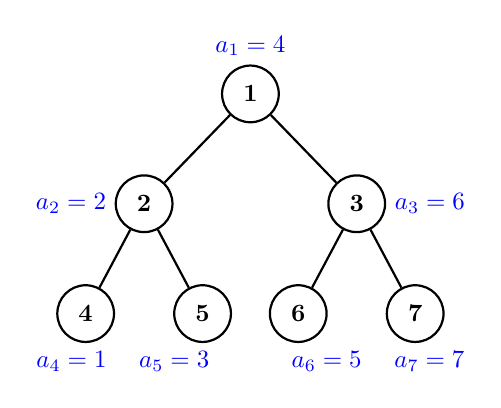
\begin{tikzpicture}[
scale=0.90,
transform shape,
level 1/.style={sibling distance=3.0cm},
level 2/.style={sibling distance=1.65cm},
level distance=1.55cm,
villager/.style={
circle,
draw=black,
thick,
minimum size=0.8cm,
font=\bfseries
},
edge from parent/.style={draw=black, thick}
]
\node[villager, label={[text=blue]above:$a_1=4$}] {1}
child {
node[villager, label={[text=blue]left:$a_2=2$}] {2}
child {
node[villager,
label={[text=blue,xshift=-2mm]below:$a_4=1$}] {4}
}
child {
node[villager,
label={[text=blue,xshift=-4mm]below:$a_5=3$}] {5}
}
}
child {
node[villager, label={[text=blue]right:$a_3=6$}] {3}
child {
node[villager,
label={[text=blue,xshift=4mm]below:$a_6=5$}] {6}
}
child {
node[villager,
label={[text=blue,xshift=2mm]below:$a_7=7$}] {7}
}
};
\end{tikzpicture}
\caption{Initial state}
\end{subfigure}\hfill%
% ---------- (b) 执行 J(1,7) 后 ----------
\begin{subfigure}[t]{0.32\linewidth}
\centering
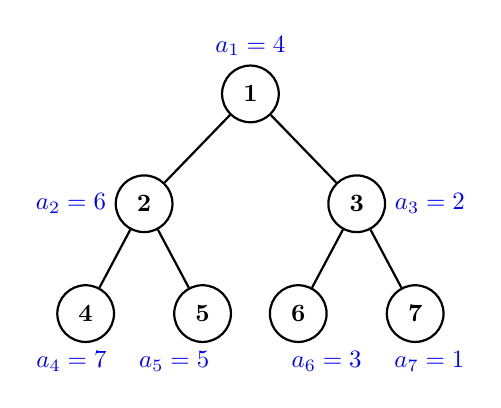
\begin{tikzpicture}[
scale=0.90,
transform shape,
level 1/.style={sibling distance=3.0cm},
level 2/.style={sibling distance=1.65cm},
level distance=1.55cm,
villager/.style={
circle,
draw=black,
thick,
minimum size=0.8cm,
font=\bfseries
},
edge from parent/.style={draw=black, thick}
]
\node[villager, label={[text=blue]above:$a_1=4$}] {1}
child {
node[villager, label={[text=blue]left:$a_2=6$}] {2}
child {
node[villager,
label={[text=blue,xshift=-2mm]below:$a_4=7$}] {4}
}
child {
node[villager,
label={[text=blue,xshift=-4mm]below:$a_5=5$}] {5}
}
}
child {
node[villager, label={[text=blue]right:$a_3=2$}] {3}
child {
node[villager,
label={[text=blue,xshift=4mm]below:$a_6=3$}] {6}
}
child {
node[villager,
label={[text=blue,xshift=2mm]below:$a_7=1$}] {7}
}
};
\end{tikzpicture}
\caption{After Judgment $(1,7)$}
\end{subfigure}\hfill%
% ---------- (c) 再执行 L(4,5) 后 ----------
\begin{subfigure}[t]{0.32\linewidth}
\centering
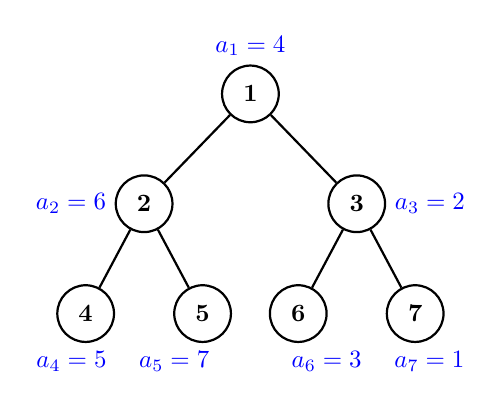
\begin{tikzpicture}[
scale=0.90,
transform shape,
level 1/.style={sibling distance=3.0cm},
level 2/.style={sibling distance=1.65cm},
level distance=1.55cm,
villager/.style={
circle,
draw=black,
thick,
minimum size=0.8cm,
font=\bfseries
},
edge from parent/.style={draw=black, thick}
]
\node[villager, label={[text=blue]above:$a_1=4$}] {1}
child {
node[villager, label={[text=blue]left:$a_2=6$}] {2}
child {
node[villager,
label={[text=blue,xshift=-2mm]below:$a_4=5$}] {4}
}
child {
node[villager,
label={[text=blue,xshift=-4mm]below:$a_5=7$}] {5}
}
}
child {
node[villager, label={[text=blue]right:$a_3=2$}] {3}
child {
node[villager,
label={[text=blue,xshift=4mm]below:$a_6=3$}] {6}
}
child {
node[villager,
label={[text=blue,xshift=2mm]below:$a_7=1$}] {7}
}
};
\end{tikzpicture}
\caption{After Lightning $(4,5)$}
\end{subfigure}

\end{figure}

For the third trident query in the first test case, after the preceding Judgment operation,
the current weights are
\[
(a_1,a_2,\ldots,a_7)=(4,6,2,7,5,3,1).
\]

Weights $4,5,6,7$ are at vertices $1,5,2,4$, respectively, so $S=\{1,2,4,5\}$.

Choose $F=1$, $x=4$, and $y=5$. Then:

\begin{itemize}
\item Vertex $1$ is an ancestor of vertex $4$.
\item Vertex $1$ is an ancestor of vertex $5$.
\item $ P(1,4)\cup P(1,5) =\{1,2,4\}\cup\{1,2,5\}=S$。
\end{itemize}

Therefore, $S$ is a \textbf{trident}.




\end{document}
